\section{Závěr}

Naše řešení se ukázalo poměrně kvalitním, kdy jsme bludištěm projeli zhruba za minutu a čtvrt po odečtení 30 s za poklad. Během řešení jsme narazili na několik problémů, které jsme museli vyřešit. Občas jsme měli problém přečíst ArucoTagy, nejspíš protože při rychlém otáčení se robot nestíhal vrátit na střed koridoru. Proto bylo zapotřebí rychlejší a agresivnější PID regulátor, který by zřejmě stále mohl být lepší. S tímto problémem jsme si vypomohli i přejitím při otáčení na časovač místo IMU. Je to sice méně robustní řešení a pokud bychom chtěli změnit rychlost otáčení, museli bychom experimentálně určit dobu otáčení, ale pro tento úkol nám výrazně zrychlilo čas.
Další problém jsme měli s příchodem dat ze senzorů. Občas nám chvíli nepřicházeli data a tudíž se robot opět vychyloval ze středu koridoru, nebo zavčas nedetekoval stěnu před sebou. Tuto chybu jsme nemohli odstranit, protože byla zřejmě způsobena sítí, ale alespoň jsme při přiblížení ke stěně přední stranou robota, lehce snížili rychlost, aby měl více času než má úplně zastavit.
\begin{comment}
\begin{figure}[h]
    \centering
    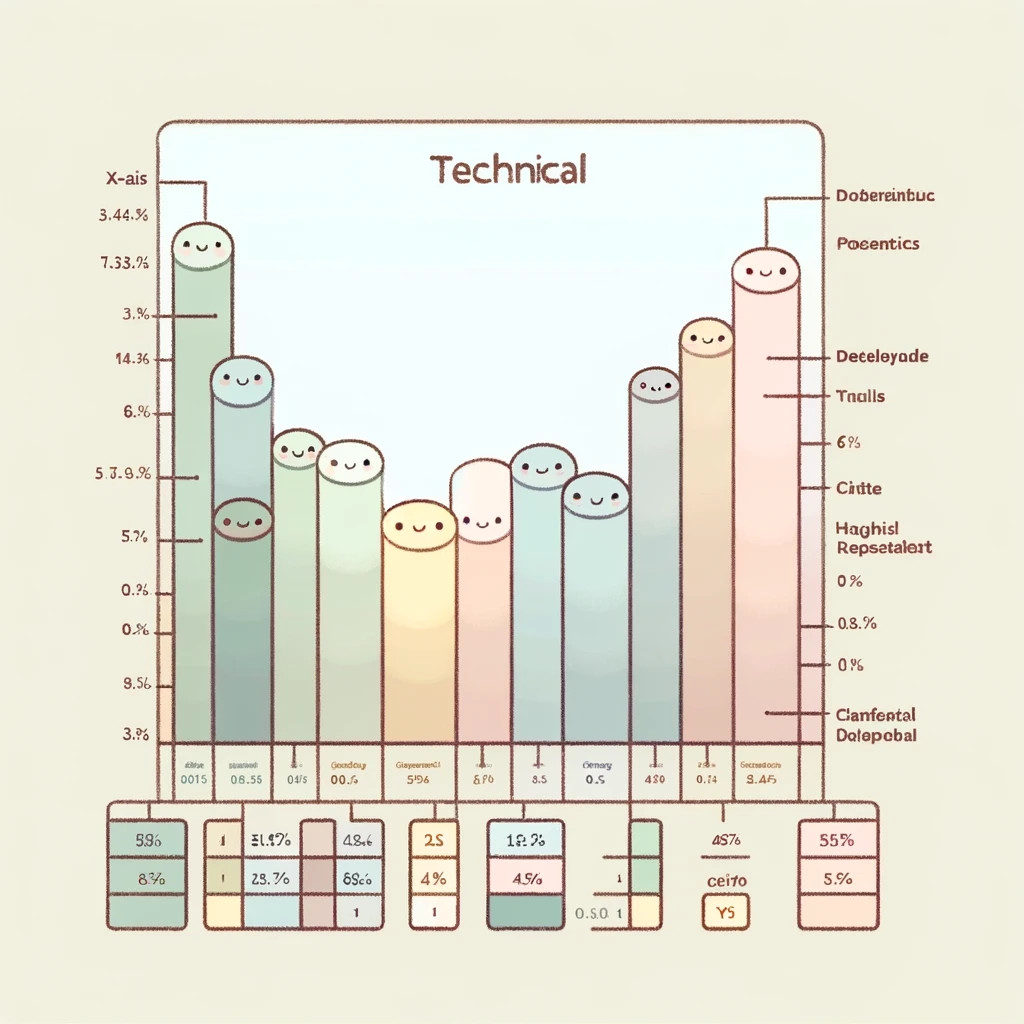
\includegraphics[width=0.45\textwidth]{images/plot.jpg}
    \caption{Plot}
    \label{fig:plot}
\end{figure}
\end{comment}